% The ideal P=(2,1+sqrt(-5)) inside Z[sqrt(-5)], drawn in C (generated).
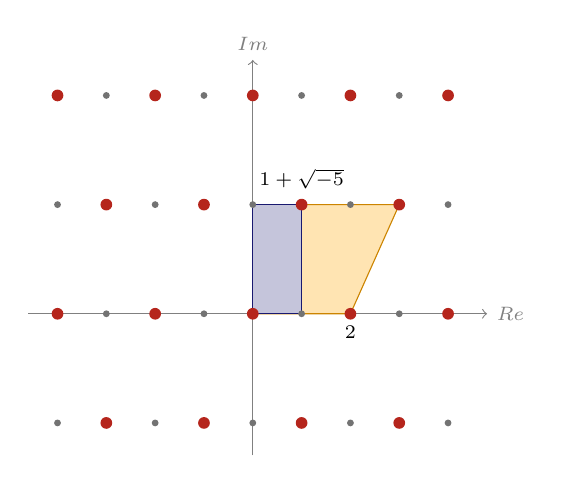
\begin{tikzpicture}[scale=0.62]
\draw[->,black!50] (-4.6,0)--(4.8,0) node[right,font=\scriptsize]{$\operatorname{Re}$};
\draw[->,black!50] (0,-2.9)--(0,5.2) node[above,font=\scriptsize]{$\operatorname{Im}$};
\fill[Orange!30,draw=Orange!80!black] (0,0)--(2,0)--(3.000,2.236)--(1,2.236)--cycle;
\fill[MidnightBlue!25,draw=MidnightBlue] (0,0)--(1,0)--(1,2.236)--(0,2.236)--cycle;
\fill[black!55] (-4.000,-2.236) circle (0.07);
\fill[BrickRed] (-4.000,0.000) circle (0.12);
\fill[black!55] (-4.000,2.236) circle (0.07);
\fill[BrickRed] (-4.000,4.472) circle (0.12);
\fill[BrickRed] (-3.000,-2.236) circle (0.12);
\fill[black!55] (-3.000,0.000) circle (0.07);
\fill[BrickRed] (-3.000,2.236) circle (0.12);
\fill[black!55] (-3.000,4.472) circle (0.07);
\fill[black!55] (-2.000,-2.236) circle (0.07);
\fill[BrickRed] (-2.000,0.000) circle (0.12);
\fill[black!55] (-2.000,2.236) circle (0.07);
\fill[BrickRed] (-2.000,4.472) circle (0.12);
\fill[BrickRed] (-1.000,-2.236) circle (0.12);
\fill[black!55] (-1.000,0.000) circle (0.07);
\fill[BrickRed] (-1.000,2.236) circle (0.12);
\fill[black!55] (-1.000,4.472) circle (0.07);
\fill[black!55] (0.000,-2.236) circle (0.07);
\fill[BrickRed] (0.000,0.000) circle (0.12);
\fill[black!55] (0.000,2.236) circle (0.07);
\fill[BrickRed] (0.000,4.472) circle (0.12);
\fill[BrickRed] (1.000,-2.236) circle (0.12);
\fill[black!55] (1.000,0.000) circle (0.07);
\fill[BrickRed] (1.000,2.236) circle (0.12);
\fill[black!55] (1.000,4.472) circle (0.07);
\fill[black!55] (2.000,-2.236) circle (0.07);
\fill[BrickRed] (2.000,0.000) circle (0.12);
\fill[black!55] (2.000,2.236) circle (0.07);
\fill[BrickRed] (2.000,4.472) circle (0.12);
\fill[BrickRed] (3.000,-2.236) circle (0.12);
\fill[black!55] (3.000,0.000) circle (0.07);
\fill[BrickRed] (3.000,2.236) circle (0.12);
\fill[black!55] (3.000,4.472) circle (0.07);
\fill[black!55] (4.000,-2.236) circle (0.07);
\fill[BrickRed] (4.000,0.000) circle (0.12);
\fill[black!55] (4.000,2.236) circle (0.07);
\fill[BrickRed] (4.000,4.472) circle (0.12);
\node[font=\scriptsize,anchor=north] at (2,-0.05) {$2$};
\node[font=\scriptsize,anchor=south] at (1,2.356) {$1+\sqrt{-5}$};
\node[font=\scriptsize,anchor=south] at (0.45,2.236) {};
\end{tikzpicture}
